\documentclass[9pt, aspectratio=169]{beamer}
\usetheme{default}

\usepackage{soul}
\usepackage{amsmath}
\usepackage{mathtools}
\usepackage{physics}
\usepackage{amssymb,amsmath,amsfonts}
\usepackage[utf8]{inputenc}
\usepackage{graphicx}
\usepackage{geometry}
\usepackage{float}
%\usepackage[autostyle=true,german=quotes]{csquotes}
\usepackage{hyperref}
\usepackage{gensymb}
\usepackage[separate-uncertainty=true]{siunitx}
\usepackage{hhline}
\usepackage{color}
%\usepackage[export]{adjustbox}
%\usepackage[nottoc,numbib]{tocbibind}
%\usepackage[super,comma]{natbib}
%\usepackage{listings}
\usepackage{blindtext}
\usepackage[version=4]{mhchem}
\usepackage{multicol}
\usepackage{multirow}
\usepackage{units}
\usepackage{braket}
\usepackage{caption}
\usepackage{subcaption}
\usepackage{url}
\usepackage{datetime}
\usepackage{chemformula}
\usepackage[export]{adjustbox}

\usepackage{xcolor}
\usepackage{xparse}

\usepackage[T1]{fontenc}
\usepackage{lmodern}
\author{Annanay Jaitly}
\title{Investigating Amplifier Measurements}
\subtitle{Task for the Multimessenger School}
%\setbeamercovered{transparent} 
%\setbeamertemplate{navigation symbols}{}
\beamertemplatenavigationsymbolsempty 

\hypersetup{
	colorlinks=true,
	linkcolor=cyan,
	filecolor=magenta,      
	urlcolor=blue,
	pdftitle={MMS_task},
}

\addtobeamertemplate{navigation symbols}{}{%
	\usebeamerfont{footline}%
	\usebeamercolor[fg]{footline}%
	\hspace{1em}%
	\insertframenumber/\inserttotalframenumber
}

%\logo{} 

\date{\today}

%\subject{} 
\begin{document}

\begin{frame}
	\titlepage
\end{frame}

%\begin{frame}
%\tableofcontents
%\end{frame}
%\begin{frame}
%	\frametitle{Overview} % Table of contents slide, comment this block out to remove it
%	\tableofcontents % Throughout your presentation, if you choose to use \section{} and \subsection{} commands, these will automatically be printed on this slide as an overview of your presentation
%\end{frame}

%\section{Introduction}
%
%\begin{frame}
%	\frametitle{Introduction}
%
%
%\end{frame}

\begin{frame}
	\frametitle{Mean Gain Curve and Deviations}

	\begin{columns}
		\begin{column}{.45\textwidth}
			\begin{itemize}
				\item The amplifiers are designed to be identical -- the mean gain curve is expected to approximate the manufacturer's ideal gain curve.
				\item The deviations from the mean gain curve are plotted in units of standard deviation at each frequency. These are symmetrically distributed about the mean gain curve.
				\item Offsets in the gain curves specific to each amplifier are visible. In the constant gain region amplifiers' gain curves lie within $\sim 2$ standard deviations or ca 5\% of the mean gain curve.
			\end{itemize}
		\end{column}

		\begin{column}{.55\textwidth}
			\begin{figure}[H]
				\centering
				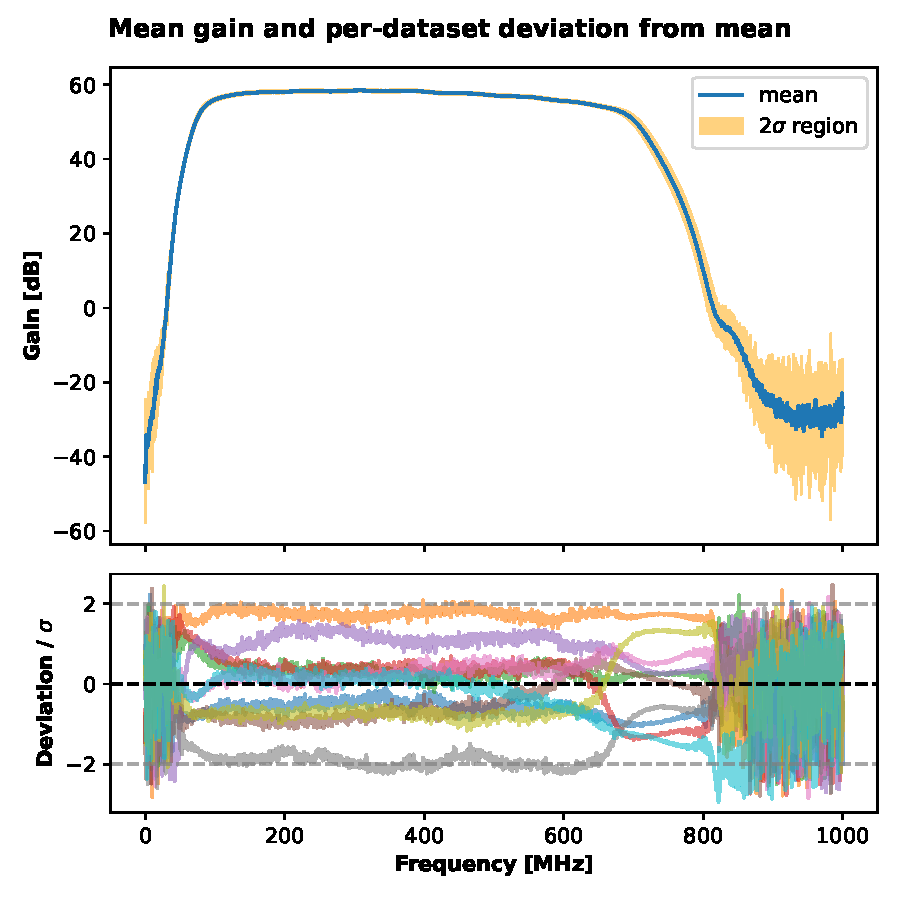
\includegraphics[width=1.0\linewidth]{../mean_and_deviation}
				\label{fig:meananddeviation}
			\end{figure}
		\end{column}
	\end{columns}


\end{frame}

\begin{frame}
	\frametitle{Zooming in on the Constant Gain Region}
	
	\begin{columns}
		\begin{column}{.45\textwidth}
			\begin{itemize}
				\item The constant gain region is approximated as the region between the extrema of the gain gradient w.r.t frequency.
				\item The offsets in the individual gain curves are more visible now.
				\item The gradient of the mean gain curve oscillates between $\pm 0.04$ dB/MHz in this region. The individual gain gradients follow the same trend in phase with the former's oscillations
			\end{itemize}
		\end{column}
		
		\begin{column}{.55\textwidth}
			\begin{figure}[H]
				\centering
				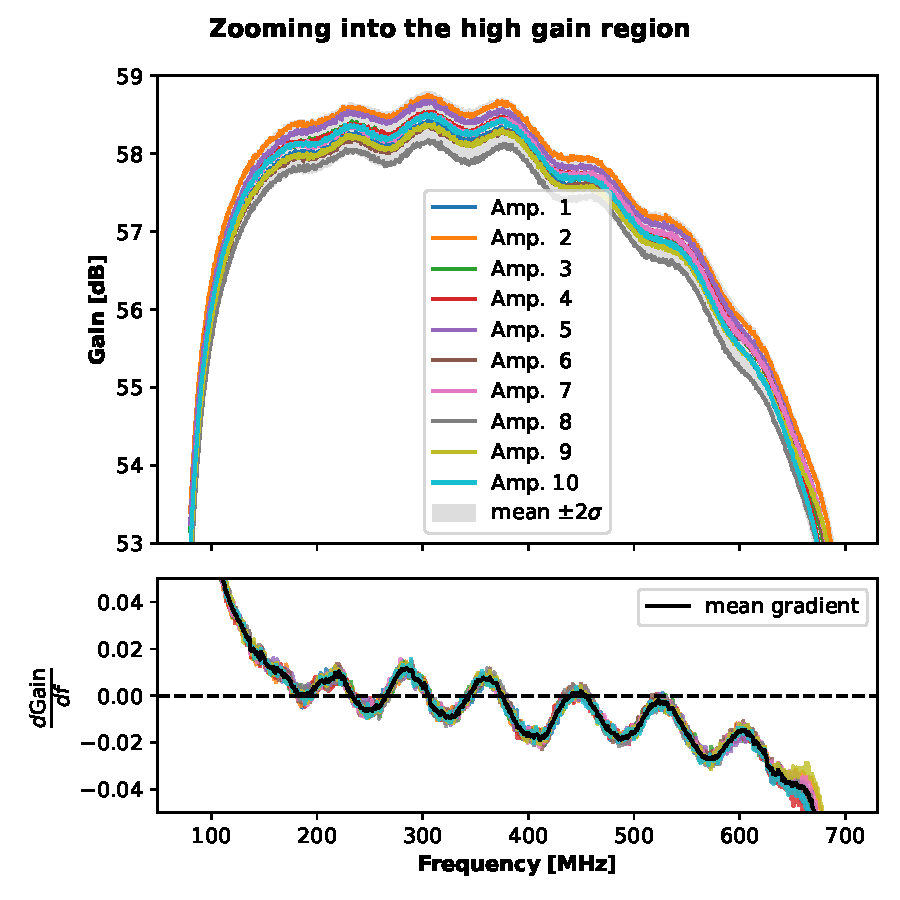
\includegraphics[width=1.0\linewidth]{../zoomed}
				\label{fig:zoomed}
			\end{figure}
		\end{column}
	\end{columns}
	
	
\end{frame}

\end{document}
